\section{Обзор}
В данном разделе представлен обзор предметной области:
основные способы реализации предметно-ориентированных языков; 
процесс отображения пользовательских интерфейсов;
существующие языки программирования общего назначения, предоставляющие
пользователям возможность декларативного описания пользовательских
интерфейсов с помощью предметно-ориентированных языков.

\subsection{Предметная область}
\subsubsection{Предметно-ориентированные языки}
\label{dsl-section}
Предметно-ориентированный язык (\textit{domain-specific language}, DSL) ---
это язык программирования с более высоким уровнем абстракции,
отражающий специфику решаемых с его помощью задач. Такой язык оперирует
понятиями и правилами из определенной предметной области~\cite{book-of-dsls}.

В отличие от языков программирования общего назначения, таких как \name{C},
\name{Python}, \name{Java}, предметно-ориентированные языки предоставляют
абстракции, адекватные решаемой проблеме, позволяя выражать решения,
написанные с их помощью, кратко и ёмко; причём в некоторых случаях
использование DSL не требует квалификации программиста.
В качестве примера DSL можно привести \name{SQL} ---  декларативный язык
программирования, применяемый для создания, модификации и управления данными в
реляционной базе данных.
Основным недостатком применения предметно-ориентированных языков является
стоимость их разработки, требующая экспертизы как в области разработки языков
программирования, так и в целевой предметной области.
Это является одной из причин того, что предметные языки редко применяются
для решения задач программной инженерии, в отличие от языков программирования
общего назначения.
Другой причиной отказа от обособленных предметных языков является тот факт,
что сочетание программной библиотеки и языка программирования общего
назначения может заменять DSL.
Программный интерфейс (\textit{Application Programming Interface},
API) библиотеки содержит специфичный для определённой
области словарь, образованный именами классов, методов и функций, доступный
всем пользователям языков программирования общего назначения, подключившим
библиотеку.
Однако, вышеприведённый подход проигрывает предметным языкам в следующих
аспектах~\cite{when-and-how-develop-dsl,dsl-spectrum-wile}:
\begin{itemize}
	\item устоявшаяся в области нотация, как правило, выходит за рамки
	ограниченных механизмов определения пользовательских операторов,
	предоставляемых языками общего назначения;
	\item абстракции определённой области не всегда могут быть
	просто отображены в конструкции языков общего назначения~\cite{dsl-traversal-transform};
	\item использование предметно-ориентированного языка сохраняет
	возможность анализа, верификации, оптимизации, параллелизации и
	трансформации в рамках конкретной области, что, в случае работы с
	исходным текстом языка программирования общего назначения, является
	более сложной задачей.
\end{itemize}

\subsubsection{Подходы к реализации предметно-ориентированных языков}
В последнее время всё больше исследований в области
предметно-ориен\-тированных языков направлены на категоризацию предметных
языков, а также выработку советов и лучших практик, отвечающих на вопросы
"когда и как?" создавать DSL для конкретной области~\cite{when-and-how-develop-dsl,study-on-preliminary-approaches-develop-dsl,spinellis-dsl-patterns}.
\paragraph{Препроцессинг}
DSL-конструкции транслируются в более низкоуровневый программный код
базового языка программирования общего назначения.
\begin{itemize}
	\item \textit{Макрокоманда}. Конструкции предметного языка представлены
	символьными именами, заменяемыми при обработке препроцессором на
	последовательность программных инструкций базового языка.
	\item \textit{Транспиляция}. Исходный код предметного языка
	транслируется в исходный код языка общего назначения.
	\item \textit{Лексическая обработка}. Трансформация предметного языка в
	язык общего назначения осуществляется на уровне лексем.
\end{itemize}

Преимуществом данного подхода является простота реализации DSL, поскольку
большая часть семантического анализа выполняется средствами базового языка.
В то же время, это является и недостатком данного подхода ввиду отсутствия
предметно-ориентированного статического анализа, оптимизаций и сообщений об ошибках.

\paragraph{Встраивание в базовый язык}
В данном подходе конструкции базового языка используются для построения
библиотеки предметно-ориен\-тированных операций. С помощью синтаксиса
базового языка задаётся диалект, максимально приближенный к определённой
предметной области.

Преимуществом данного подхода является полное переиспользование компилятора или интерпретатора базового языка для построения DSL. Основными недостатками
являются сообщения об ошибках, соответствующие спецификации базового языка,
и ограниченная синтаксическая выразительность, обусловленная
существующим синтаксисом базового языка.

\paragraph{Самостоятельный компилятор}
В данном подходе для создания DSL используются методы построения
компиляторов или интерпретаторов. В случае компилятора, конструкции
предметного языка транслируются во внутреннее представление компилятора, а
статический анализ производится над спецификацией DSL. В случае
интерпретатора, конструкции предметного языка распознаются и выполняются
в ходе цикла выборки-распознавания-исполнения (fetch-decode-execute cycle).

Преимуществами данного подхода являются приближенные к предметной
области синтаксис языка и сообщения об ошибках. Серьёзным недостатком
является необходимость создания нового компилятора или интерпретатора
предметного языка.

\paragraph{Компилятор компиляторов}
Данный подход схож с предыдущим за исключением того, что все или некоторые
стадии компиляции выполняются с использованием \textit{компилятора компиляторов} --- программы, воспринимающей синтаксическое или семантическое
описание языка программирования и генерирующей компилятор для этого языка.

Преимуществом подхода является снижение расходов на создание компилятора
предметного языка. Ограниченность итогового DSL возможностями используемого
компилятора компиляторов, а также сложность проработки предметного языка в
деталях, что может быть критично для достижения определённого уровня
производительности и близости сообщений об ошибках к предметной области,
составляют недостатки данного подхода.

\paragraph{Расширение существующего компилятора}
Компилятор языка программирования общего назначения расширяется
предметно-ориенти\-рованными правилами оптимизации и/или генерации кода.

В сравнении с предыдущим, данный подход менее трудоёмок из-за возможности
переиспользования частей существующего компилятора. Однако, стоит отметить,
что расширение существующего компилятора может оказаться сложной задачей,
для выполнения которой необходима поддержка расширений со стороны
компилятора языка общего назначения, а также минимизация пересечений
синтаксиса и семантики базового и предметного языков.

\paragraph{Использование готовых инструментов}
Существующие инструменты и нотации адаптируются под конкретную предметную
область. Примером такого подхода являются DSL, основанные на нотации
\name{XML}. В большинстве случаев предметные языки, полученные данным
способом, плохо подходят для их использования людьми в ручном режиме.

\newpage
\subsubsection{Отображение пользовательского интерфейса}
В данном разделе представлен один из способов
отображения пользовательских интерфейсов, использующийся в популярных
средствах разработки приложений~\cite{flutter-homepage,swift-homepage,
vuenative-homepage,reactnative-homepage}. Графическая подсистема
языка \name{Accord} основана на схожем подходе. Стоит также отметить, что
далее будут рассмотрены лишь базовые принципы построения и отображения
интерфейсов, которых должно быть достаточно для объяснения тех или иных
оптимизационных решений, принятых в данной работе.

Задачей построения и отображения пользовательского интерфейса занимается
так называемый движок рендеринга или отрисовки (\textit{ren\-dering engine})
--- программное обеспечение, получающее изображение по какой-либо модели.
Здесь \textit{модель} --- это описание любых объектов или явлений на строго
определённом языке или в виде структуры данных.

На рисунке~\ref{render-pipeline} представлен схематичный шаг алгоритма
рендеринга пользовательского интерфейса. Так, отрисовка кадра \textit{N}
состоит из нескольких последовательных этапов:
\begin{enumerate}
	\item построение дерева компонентов по текущему состоянию
	пользовательского интерфейса. \textit{Дерево компонентов} ---
	древовидная структура данных, элементами которой являются
	высокоуровневые компоненты интерфейса. Примером такого дерева
	может являться \name{DOM} (от англ. \textit{Document Object Model} ---
	объектная модель документа), использующийся в современных веб-браузерах.
	\item построение дерева элементов по дереву компонентов. \textit{Дерево
	элементов} --- древовидная структура данных, изоморфная дереву
	компонентов, элементами которой являются структуры данных движка
	рендеринга.
	\item построение дерева рендеринга по дереву элементов. \textit{Дерево
	рендеринга} --- древовидная структура данных, содержащая в себе только
	необходимые для непосредственно рендеринга элементы интерфейса. Говоря
	о переходе между деревом элементов и деревом рендеринга как об
	отображении, можно сказать, что не все узлы дерева элементов имеют
	свой образ в дереве рендеринга. Так же стоит отметить, что узлы дерева
	рендеринга содержат в себе низкоуровневую информацию, такую как
	относительные координаты элемента в виртуальном пространстве движка
	отрисовки.
	\item размещение и отрисовка: перевод всех относительных свойств
	элементов в абсолютные, например, перевод относительных координат
	элемента в виртуальном пространстве движка отрисовки в координаты
	элемента на экране реального устройства; формирование запроса к
	аппаратуре для отрисовки интерфейса.
\end{enumerate}

\begin{figure}[h]
\centering
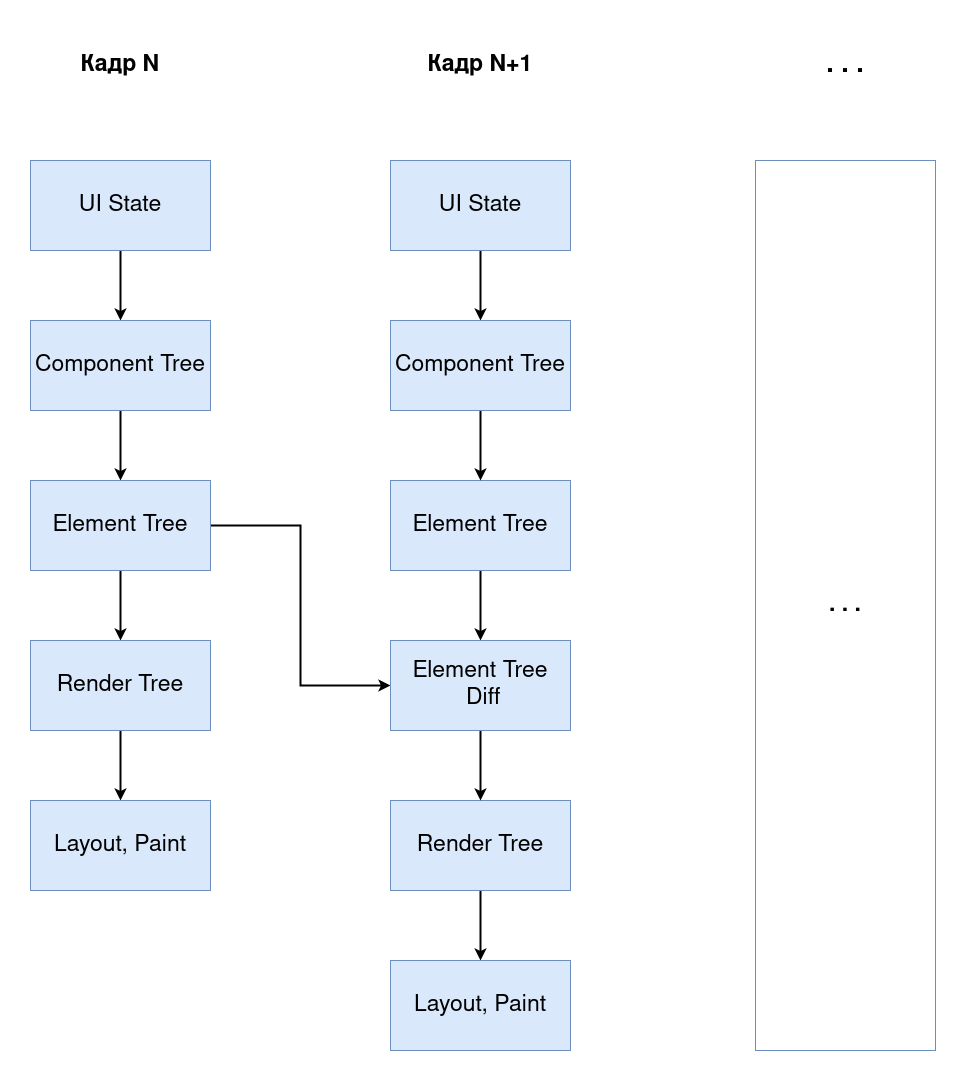
\includegraphics[width=\linewidth,height=0.9\linewidth,keepaspectratio]{resources/ui-render-pipeline.png}
\caption{Схематичный шаг алгоритма рендеринга пользовательского интерфейса}
\label{render-pipeline}
\end{figure}

Процесс отрисовки кадра \textit{N+1}, в свою очередь, повторяет
вышеописанный алгоритм за исключением следующего: дерево рендеринга
перестраивается на основании разницы между деревьями элементов текущего и
предыдущего кадров.
Подобное дополнение позволяет значительно повысить производительность
всего графического конвейера за счёт переиспользования вычислений,
хранящихся в дереве рендеринга предыдущего кадра.

\subsection{Существующие решения}

\subsection{Вывод}
